\newpage % Rozdziały zaczynamy od nowej strony.
\section{Gra strategiczna Statki – podstawowe zasady i historia}

\subsection{Historia gry}
\indent\ Gra Statki, znana również jako "Battleships", to popularna gra strategiczna, której korzenie sięgają początku XX wieku. Jest to gra turowa dla dwóch graczy, którzy starają się zatopić flotę przeciwnika oddając na zmianę strzały na planszę przeciwnika. Gracze nie widzą planszy przeciwnika, po każdym oddanym strzale dostają jedynie informację zwrotną, czy trafili w statek.
\\ \indent Pierwsze wersje gry "Statki" były grami papierowymi, które były popularne wśród żołnierzy w trakcie I Wojny Światowej. Do gry potrzebne były jedynie 2 kartki oraz ołówek, więc można było w nią grać właściwie wszędzie. \cite{historyWiki}
\\ \indent Od lat 30 XX wieku, dostępne były komercyjne wersje gry - gracze mogli kupić gotowe papierowe plansze do gry, aby nie musieć własnoręcznie ich rysować. W 1967 firma Milton Bradley zaczęła produkować prawdopodobnie najbardziej znaną wersję gry, składającą się z plastikowych planszy oraz statków. \cite{historyWiki} \cite{museumOfGames}

\begin{figure}[!h]
    \label{fig:milton-bradley-game}
    \centering 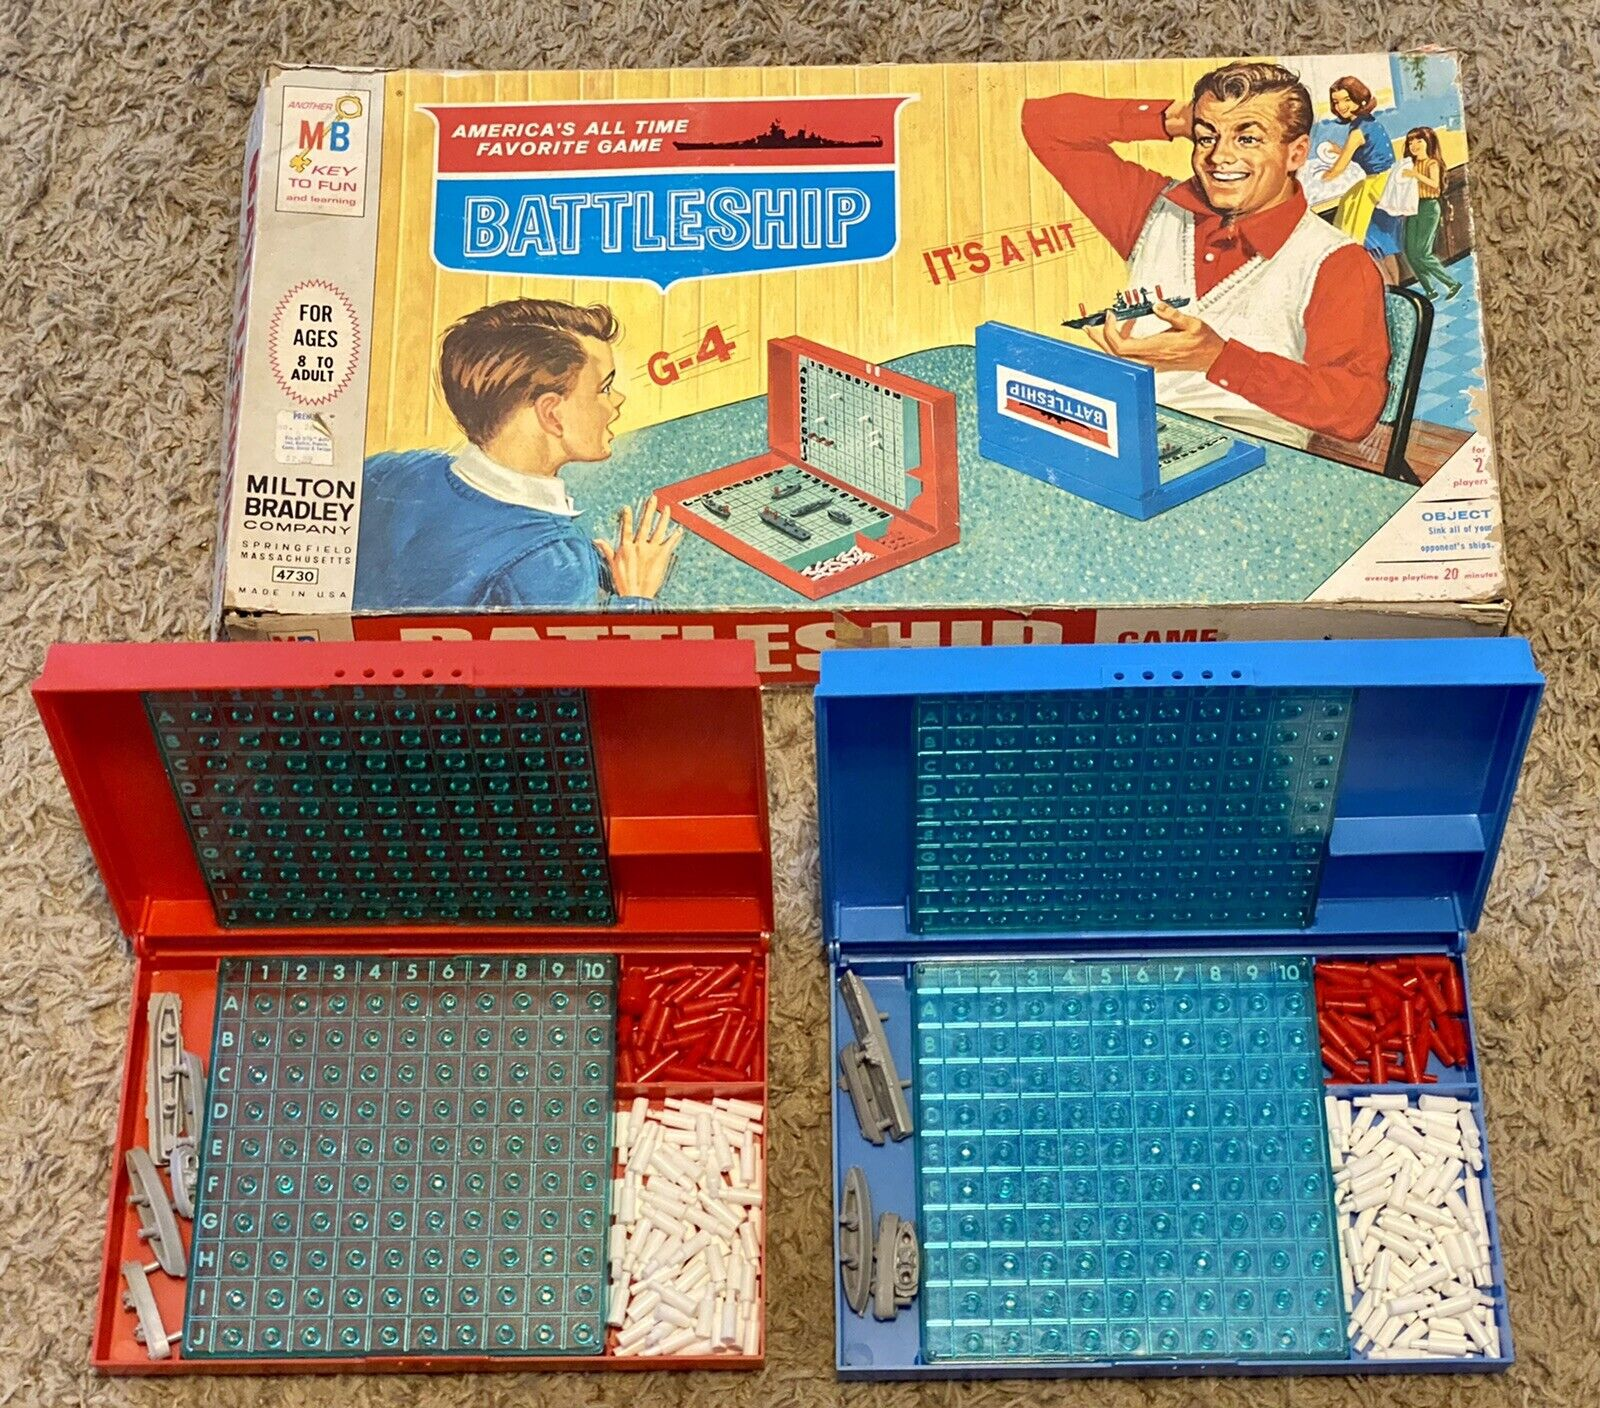
\includegraphics[width=0.8\linewidth]{img/milton_bradley_game.jpg}
    \caption{Gra Battleship wyprodukowana przez firmę Milton Bradley \cite{eBay}.}
\end{figure}

 \indent Z biegiem lat gra Statki ewoluowała, przyjmując różne formy. W latach 70. XX wieku pojawiła się pierwsze wersja elektroniczna, dostępna na komputerach Z80 Compucolor, napisana w języku BASIC. Wraz z rozwojem PC, zaczęło pojawiać się coraz więcej wersji gry.\cite{historyWiki} \cite{museumOfGames} .

 \begin{figure}[!h]
    \label{fig:commodore_64}
    \centering 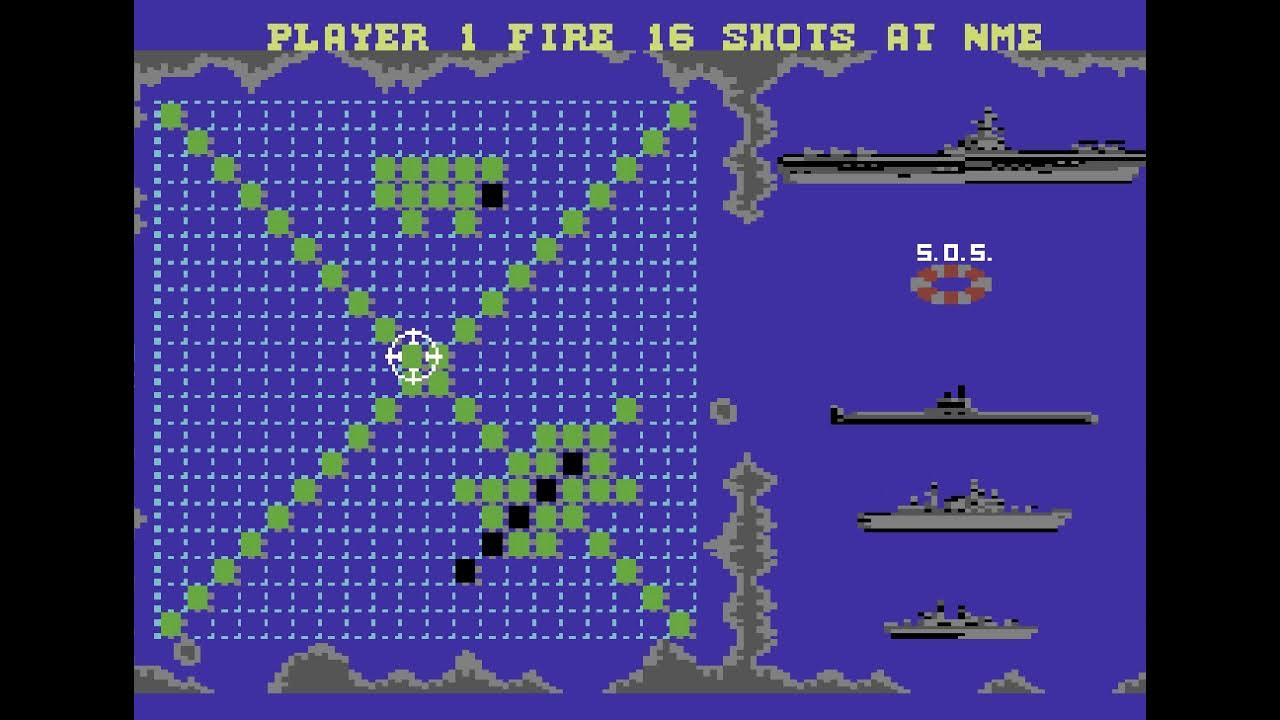
\includegraphics[width=0.8\linewidth]{img/commodore_64.jpg}
    \caption{Ujęcie z gry \emph{Battleship} dostępnej na komputerze Commodore 64 \cite{commodore64}.}
\end{figure}

\indent Gra Statki jest znanym elementem kultury popularnej na całym świecie, na jej podstawie w 2012 powstał nawet film "Battleship".
\subsection{Zasady}
\indent\ Zasady gry Statki różnią się w zależności od wersji. Zasady przyjęte w niniejszej pracy:
\begin{itemize}
  \item Gracze mają do dyspozycji po jednym statku o danej długości, zaczynając od jednomasztowca, kończąc na pięciomasztowcu.
  \item Dany statek musi leżeć w linii prostej (nie może na przykład być "złamany" i tworzyć literę L)
  \item Plansza ma wymiary 10 na 10.
  \item Gracz może wybrać czy statki mogą się ze sobą stykać bokami lub rogami. Ma to na celu dodanie dodatkowej zmiennej do analizy skuteczności algorytmów.
\end{itemize}

Różnorodność zasad to być może coś, co przyczyniło się do popularności tej gry - gracze mogą zmieniać zasady, tak aby rozgrywka była dla nich jak najciekawsza. Gra ograniczona wieloma zasadami, takimi jak to że statki nie mogą sąsiadować, prowadzi do bardziej analitycznej rozgrywki - gracze mogą eliminować z rozważań pola, na których zgodnie z zasadami nie mogą znajdować się statki. Gdy nie ma zasad ograniczających rozstawienie statków, gra robi się dużo bardziej losowa.